\section{Selection}
\label{sec:RKst_selection}

The selection process, described in this section, is divided into several steps:
\begin{itemize}
\item first of all candidates have to fall into the detector acceptance, produce hits and be selected
on the basis of quality features, such as $\chi^2$ of tracks and vertices and basic kinematic cuts.
This stage is called ``stripping". Furthermore, it is required that the events are triggered by specific
trigger lines and cuts are applied to remove backgrounds from specific decays.
All these first three steps are referred to as ``pre-selection";
\item secondly, particle identification requirements are applied to remove part of misreconstructed
background and clear the way for the last step;
\item in the final step a neural network is used to remove combinatorial background.
\end{itemize}
%
In order to minimise the systematic uncertainties the same selection requirements are used to select 
the rare signal candidates and the relative charmonium channel, a part from the \qsq cuts which serve
to distinguish them. To identify the $\Bz \to\Kstarz(\jpsi\to \mumu)$ channel a dilepton mass
interval of 100~\mevcc~around the nominal \jpsi peak~\cite{PDG2014} is selected.
On the other hand it is not possible to use a narrow cut on the \qsq of $\jpsi(ee)$ channel as its
distribution is characterised by a long radiative tail at low masses due to bremsstrahlung radiation.
Furthermore, a cut in \qsq distorts the 4-body $m(K\pi ee)$ mass distribution and it is important to
be able to fit a wide mass range to constrain the backgrounds. For these reasons the interval to select
$\Bz \to\Kstarz(\jpsi\to \epem)$ candidates is chosen to go as low as possible without overlapping with
the rare channel interval. The electron resonant channel is therefore selected in the interval
$6-11~\gevgevcccc$. Figure~\ref{fig:2D_q2_B0mass} shows two-dimensional distributions
of \qsq versus 4-body invariant mass for candidates passing the full selection.
Horizontal bands can be clearly seen at \qsq values corresponding to the \jpsi and \psitwos resonances.
On the plot for muons it is also evident a vertical band which corresponds to rare decay of interest.

\begin{figure}[t!]
\centering 
\includegraphics[width=1.\textwidth]{RKst/figs/electron_B0jpsi2D_selected.pdf}
\includegraphics[width=1.\textwidth]{RKst/figs/muon_B0jpsi2D_selected.pdf}
\caption{Two-dimensional distributions of \qsq versus 4-body $m(K\pi\ell\ell)$
invariant mass for the electron (top) and muonic (bottom) channels in 2012 data.}
\label{fig:2D_q2_B0mass}
\end{figure}


\subsection{Trigger and Stripping }
\label{sec:RKst_trigstripping}

Events are triggered for the $\mu\mu$ and the $ee$ channels by the trigger lines
reported in Tab.~\ref{tab:RKst_triglines}, where the logical $and$ of L0, HLT1 and HLT2
lines is required and the logical $or$ of the lines on the same level. The candidates are
required to be triggered-on-signal (TOS) for most of the stages, namely
it is required for the particle which triggered to be one of the particles used to build the signal candidates.
Only for \verb!L0Global!, used in the electron case, we require a trigger-independent-of-signal (TIS),
this is aimed to collect all the possible statistics for the electron channels, which are the most challenging.
The \verb!L0Muon! trigger requires hits in the muon detector, while \verb!L0Electron! and \verb!L0Hadron! use information
from the calorimeters; \verb!HLT1TrackAllL0! adds information from the trackers and
triggers if the L0 decision is confirmed; finally, \verb!HLT2Topo[2,3]BodyBBDT! uses a full reconstruction 
of the event and a neural network trained on events with a specific topology in order to detect specific decay structures.
%More information about the muon triggers can be found at Sec.~\ref{sec:Lb_trigger}.

\begin{table}[h!]
\begin{center}
\caption{Summary of the trigger lines used to select the $\mu\mu$ and the $ee$ channels.
Where not explicitly indicated, the lines are required to be TOS.}
\begin{tabular}{c|c}
$\mu\mu$ candidates &  $ee$ candidates \\
\hline
	L0Muon		& L0Electron\\
				& L0Hadron\\
				& L0Global (TIS)\\
\hline
	Hlt1TrackAllL0				& Hlt1TrackAllL0 \\
	Hlt1TrackMuon				&	 \\
\hline
	Hlt2Topo[2,4]BodyBBDT 		& Hlt2Topo[2,4]BodyBBDT \\
	Hlt2TopoMu[2,4]BodyBBDT 	& Hlt2TopoE[2,4]BodyBBDT \\
	Hlt2DiMuonDetachedDecision	&							\\
\end{tabular}
\label{tab:RKst_triglines}
\end{center}
\end{table}

For the electron channels the L0 lines have different properties, therefore the analysis 
is performed separately for three categories of events, depending on the L0 trigger that fired 
them. These categories are defined to be exclusive in the following way:
%
\begin{itemize}
\item {\bf L0E}: events triggered by at least one of the electrons in the signal candidate (\verb!L0Electron_TOS!);
\item {\bf L0H}: events triggered by at least one of the hadrons in the signal candidate and not by L0Electron (\verb|L0Hadron_TOS && !L0Electron_TOS|);
\item {\bf L0I}: events triggered by particles not in the signal candidate and not by the previous cases 
(\verb|L0_TIS && !(L0Electron_TOS |\verb!|| L0Hadron_TOS)!).
\end{itemize}

The majority of the selected events falls in the L0E category, while
the L0H category is more efficient at low \qsq were the \Kstarz has more momentum.
Because L0I is defined to be independent of the signal candidate, the corresponding
signal efficiency is the same in the rare and resonant cases and cancels out in their ratio.

Candidates are then required to pass the kinematic and quality cuts summarised in Tab.~\ref{tab:RKstripping}. 
The meaning of the variables in the table was already explained in Sec.~\ref{sec:Lb_selection}.
Loose PID cuts are applied in preselection to limit the size of the samples, while tighter cuts are applied
in a second stage. A large mass window is kept around the \Bz peak in order to be able
to use the sideband to train the multivariate analysis and to constrain the backgrounds.
%
%In the table $IP_{\chi_2}$ is defined as the projected distance from the vertex divided by its uncertainty, for example $IP^B_{\chi_2}(primary) > 4$ means
%that the B vertex is 2 standard deviations away from the primary vertex.
%Another quantity used is a pointing variable defined as the angle between the direction of the particle momentum and the flight direction from its mother vertex, called DIRA.
%This allows the selection of particles with well-defined primary vertices.
%%$GhostProb$ is the probability, estimated from the reconstruction algorithm, for the track to be a ghost. 
%Loose PID cuts are applied in preselection to limit the size of the samples, while tighter cuts are applied
%in a second stage. To quantify the PID of a particle the pion is used as a reference point and a Log-Likelihood
%variable is used. Therefore the {\verb PID } variable reported in the table is given in terms of the difference between
%the Log-Likelihood of the particle of a given type and a pion. This is called Delta Log-Likelihood (DLL).
%For example:
%\begin{equation}
%\verb!PID!_K = \text{DLL}_{K-\pi} = \log(\mathcal{L}_K) - \log(\mathcal{L}_\pi)
%\end{equation}
%
\begin{table}[]
\begin{center}
\caption{Summary of stripping requirements used for the central and high \qsq regions. }
\begin{tabular}{|c|c|}
\hline
Particle &  Requirements \\
\hline
%\multirow{2}{*}{ All final}
%       			&   track $\chi_2/\text{ndf} < 3$ \\
%       			&   {\verb GhostProb } $< 0.4$ \\
%\hline
$\pi$			& $\chisqip(primary) > 9$ \\      			
\hline
\multirow{3}{*}{K}
      			& {\verb PID }$_K > -5$ \\
       			& $\chisqip(primary) > 9$ \\
       			& {\verb hasRICH }  \\
 \hline
\multirow{4}{*}{ \Kstarz }
       			& $\pt > 500$ \mevc \\
       			& $|m - m_{\Kstarz}^{PDG}| < 300(????)$ \mevcc  \\ %300 in stripping but then we restrict it to 100
       			& $\chisqip(primary) > 9$ \\
       			& Origin vertex $\chi_2/\text{ndf} < 25$ \\
\hline
\multirow{3}{*}{ $\mu$ }
       			& $\pt > 300$ \mevc \\
       			& $\chisqip(primary) > 9$ \\
       			& i{\verb sMuon }\\  %RequiresDet='MUON'
%       		& hasMuon \\
\hline
\multirow{4}{*}{ $e$ }
       			& $\pt > 300$ \mevc \\
       			& $\chisqip(primary) > 9$ \\
       			& {\verb hasCalo }\\ %RequiresDet='CALO'
       			& $PID_e > 0$ \\
\hline
\multirow{4}{*}{ $\ell\ell$ }
				& $m < 5500$ \mevcc \\
			  	& End vertex $\chi^2/\text{ndf} < 9$ \\
			  	& Origin vertex $\chi^2$ separation $> 16$ \\
%			  	& $\chisqip(primary) > 0$ \\
\hline
\multirow{4}{*}{ $B^0$  }
 %      & $| m - m_{B^0}^{PDG}| < 600$ \mevcc  \\
       			& {\verb DIRA } $> 0.9995$ \\ 
       			& End vertex $\chi^2/\text{ndf} < 9$ \\
     			& $\chisqip(primary) < 25$ \\
     			& Primary vertex $\chi^2$ separation $> 100$ \\
\hline
\end{tabular}
\label{tab:RKstripping}
\end{center}
\end{table}
%
Track and vertex quality cuts are also applied using the $\chi^2_{track}/\text{ndf}$, 
{\verb GhostProb }, and $\chi^2_{vtx}/\text{ndf}$
variables. The {\verb GhostProb } quantity describes the probability of a track being fake.
By construction cutting at 0.4 removes $(1 - 0.4)\cdot 100 = 60\%$ of fake tracks.
For details about the definition of the variables used see Ref.~\cite{Loki_twiki}.

\subsection{PID}
\label{sec:PID}

After preselection there still are high levels of misreconstructed background.
In particular, as the ID of kaons and pions are not constrained, the samples
still contain both ID combinations for most candidates, therefore tighter PID cuts are applied.
In the LHCb analysis framework the particle identification probability can be quantified
using the ``{\verb ProbNN }" variables~\cite{ProbNNs_pres}. These variables are the output
of a neural network which takes as input information from the calorimeters, the RICH detectors
the muon system and the tracking system. Unlike the DLL variables (see Sec.~\ref{sec:PID_perf})
the {\verb ProbNN } are bound from 0 to 1 and can be therefore directly be interpreted as probabilities.
For example {\verb ProbNNk } is the probability for a reconstructed particle to be a kaon.
Two tunes of the {\verb ProbNN } variables, labelled V2 and V3, are available.
Tune V3 was shown to be optimal for positive ID, while tune V2 was found to be optimal
for background rejection and therefore it is used to quantify the mis-ID probability.
%
\begin{figure}[h!]
\centering 
\includegraphics[width=0.48\textwidth]{RKst/figs/muon_PID.pdf}
\includegraphics[width=0.48\textwidth]{RKst/figs/electron_PID.pdf}
\caption{Correct ID probability distributions for muons (left)
and electron (right) in 2012 data.}
\label{fig:e_mu_pid}
\end{figure}
%
\begin{figure}[h!]
\centering 
\includegraphics[width=0.48\textwidth]{RKst/figs/kaon_PID.pdf}
\includegraphics[width=0.48\textwidth]{RKst/figs/pion_PID.pdf}
\caption{On the horizontal axis of these plots is shown the correct ID
probabilities for kaons (left) and pions (right), while the vertical
axis show the mis-ID probability.}
\label{fig:k_pi_pid}
\end{figure}
%
Figure \ref{fig:e_mu_pid} shows distributions of the correct ID variables
in the 2012 data sample while Fig.~\ref{fig:k_pi_pid} shows in a two-dimensional
plane the probability of correct identification and mis-identification of kaons and pions.
These plots are characterised by clear peak at maximal ID probability and minimal mis-ID
probability, corresponding to particles to which a well defined identification can be assigned.
%
In order to maximise the power of the PID requirements probabilities of correct ID 
and mis-ID are combined using the following cuts:
%
\begin{center}
\begin{tabular}{lcl}
$\pi$ &\to  & $\verb!ProbNNpi-V3! \times (1 - \verb!ProbNNk-V2!) \times (1 - \verb!ProbNNp-V2!) > 0.1$ \\
$K$   &\to  & $\verb!ProbNNk-V3! \times (1 - \verb!ProbNNp-V2! ) > 0.05$ \\ 
$\mu$ &\to  & $\text{min}(\verb! ProbNNmu-V3! , \verb! ProbNNmu-V3 !) > 0.2$  \\
$e$   &\to  & $\text{min}(\verb! ProbNNe-V3! , \verb! ProbNNe-V3 !) > 0.2$ \\
\end{tabular}
\end{center}
%
In the first formula, for example, {\verb ProbNNpi } is the probability of correctly identifying the
pion as a pion, while {\verb ProbNNk } is the probability of mistaking it for a kaon.
Therefore by maximising the quantity ``{\verb ProbNNpi } $\times$ (1 - {\verb ProbNNk })",
one can maximise the correct ID probability and minimise at the same time the mis-ID probability.
%In the kaon case we do not use requirements on the $K\to\pi$ mis-ID probability
%because this cut was found to be unacceptably inefficient.


\subsection{Peaking backgrounds }

Backgrounds due to specific decays usually peak in some variable because of their
distinctive kinematic properties and therefore they can be removed without significant
signal efficiency loss. The following sections describe the main sources of peaking background.
The same cuts are applied to the muon and electron channels, unless specified.

\subsubsection{Charmonium vetoes}

Charmonium resonances such as \jpsi and \psitwos peak in \qsq.
The choice of \qsq binning described in Sec.~\ref{sec:RKst_q2_choice}
constitutes a natural veto for these decays. Simulated events were used
to check if resonant candidates leak inside the \qsq intervals chosen for
the rare channel analysis. For the muonic channels the leakage is negligible
as the peaks are sharper due to a better resolution and muons emit fewer
bremsstrahlung photons, resulting in shorter radiative tails.
The electronic channels are instead  characterised by
a worse resolution and at the same time electrons can radiate 
several bremsstrahlung photons, yielding long tails at low \qsq.
Analysing Monte Carlo events it was found that 1.3--2\% (depending on
the trigger category) of \mbox{$\Bz\to\Kstar(\jpsi\to\ee)$} candidates leak into the 
$1.1 < \qsq < 6$~\gevgevcccc interval and 1.8\% of \psitwos events leak above 
15~\gevgevcccc. The contribution from these candidates is modelled in the fit. 


\subsubsection{$\phi$ veto}

It can happen that a kaon from the decay $B_s \rightarrow \phi \ll$, where the $\phi$ decays in two kaons,
is mis-identified as a pion and therefore causes the $\phi$ to be reconstructed as a $\Kstarz$. This results in
a candidate with a value of $m(K\pi)$ that is less than the nominal \Kstarz mass but still high enough to
pass the selection requirements. Figure~\ref{fig:phiplots} shows the plot of $m(K\pi)$ versus
$m(K\pi \ell\ell)$, where the kaon mass hypothesis is assigned to the pion. A peak can clearly be seen
around the $\phi$ mass (1020~\mevcc).
To remove this background only candidates with $m_{K(\pi\rightarrow K)} > 1040$~\mevcc) are selected.
This results in a 98\% background rejection while keeping a 99\% signal efficiency.
%This cut could be further optimised using PID information. On the other hand LHCb simulation 
%struggles modelling the PID variables correctly. Therefore using PID in these cuts would
%add systematic uncertainties without significantly improving the signal efficiency which is already 99\%.
The $\phi$ could also constitute a background when it decays into two leptons but the
branching ratio of this decay is small compared to the one into kaons and this
contribution is taken into account by the choice of the \qsq intervals (see Sec.~\ref{sec:RKst_q2_choice}).

\begin{center}
\begin{figure}[h!]
\centering 
\includegraphics[width=0.48\textwidth]{RKst/figs/RKst/phi.pdf}
\includegraphics[width=0.48\textwidth]{RKst/figs/RKst/Kmumu.pdf}
\caption{ (left) Distribution of 2011 data events as a function of the variables $(m_{K(\pi\rightarrow K)})$ 
and $(m_{K(\pi\rightarrow K)\mu\mu})$, where $\pi\rightarrow K$ means that the kaon mass is given 
to the pions too. (right) The invariant mass distribution of the three-body system $(K\mu\mu)$,
where the peak due to the $B^+ \to K^+ \mumu$ decay is visible. }
\label{fig:phiplots}
\end{figure}
\end{center}


\subsubsection{$\Bu \to K^+ \ll$ plus a random pion}

$\Bu \to K^+ \ll$ decays can contaminate the upper \Bz mass sideband if they are combined
with a soft pion from somewhere else in the event and therefore reconstructed as a \Bz decay.
Similarly a kaon can be mis-identified as a pion and combined with an other kaon in the event.
Figure~\ref{fig:phiplots} shows the invariant mass distribution of the three-body $K\mumu$ system,
$m(K\mu\mu)$. This is characterised by a narrow peak at the $\Bu$ mass. Since these
candidates have $m(K\pi\ell\ell) > 5380$~\mevcc~there is no contribution under the \Bz peak,
but they can cause problems when using sidebands events to train the neural network.
An effective veto for this decay was found to be max$(m_{K\ell\ell},m_{(K\to\pi)\ell\ell}) < 5100$~\mevcc,
which results in 95\% background rejection while keeping 99\% signal efficiency.

\subsubsection{$\Lambda_b$ decays}

$\Lb\to\jpsi\Lz$ decays are unlikely to be reconstructed as $\Bz \to \Kstarz \ll$ because
the \Lz is long-lived and decays further in the detector with a separate vertex.
However, simulated events were used to check how many candidates fall into the \Bz samples, which results to be negligible. 
The $\Lb\to\jpsi pK$ decay, when the proton is mis-identified, can instead contribute more easily since the $m(pK)$ is above the \Lz threshold
and therefore they must come from $\Lz^*$ resonances, which are not long-lived. This background is already
reduced by the PID requirements but a non-negligible contribution is still expected, 
%in the $\mu\mu$ sample
which is modelled in the fit.

%\subsubsection{\BdToDee}

%A specific requirement is applied to remove the background coming from the \decay{\Bd}{\Dm\ep\nu} decay in which the \Dm in turn decays semileptonically to $\Kstarz\en\nu$. 
%This decay has a branching ratio four orders of magnitude larger than \BdToKstee in the low-\qsq region and it may pass the selection requirements when the two neutrinos carry a very low momentum. 
%This cut, developed for the angular analysis, uses the angle $\theta_\ell$ which is defined as the angle between the direction of the \ep (\en) in the di-electron rest frame and the direction of the di-electron in the \Bd (\Bdb) rest frame.  
%Low momentum neutrinos demand the \Dm and the \ep to be almost back-to-back in the \Bd rest frame giving the \ep a relatively large energy compared to the \en. 
%As a consequence, the direction of the \ep is close to the direction of the di-electron pair, thus the $\theta_\ell$ angle is close to 0. 
%This explains why the distribution of background selected in data with an invariant mass cut of $m(\Kstarz\epem) < 4800~\mevcc$ is asymmetric towards higher $ \cos (\theta_\ell)$ values as it can be seen in Fig.~\ref{fig:Denu_background} (\emph{left}). 
%The cut is chosen to be $|\cos (\theta_\ell) |< 0.8$, and is not applied in the high-\qsq bin.
%The percentage of \BdToeeKst signal events lost applying this cut is quite low, about $10\%$ according to MC. 

%\begin{figure}[t!]
%\centering
%\includegraphics[width=0.48\textwidth]{figs/Background/CosThetaL_background.pdf}
%\includegraphics[width=0.48\textwidth]{figs/Background/KstareMass_background.pdf}
%\caption{Distribution of (left) $\cos (\theta_\ell)$ and of (right) the $m(\Kstarz e)$ invariant mass, where the \BdToDee background is selected by requiring $m(\Kstarz\epem) < 4800\mevcc$. The red distribution corresponds to events with $| \cos ( \theta_\ell ) | > 0.8$.}
%\label{fig:Denu_background}
%\end{figure}

%In the muon channels the background from \BdToDmm decays is suppressed by the choice of the fitting range.


%\subsubsection{\BdToKstGee}
%For the low-\qsq region, a potentially dangerous peaking background is due to the \BdKstGam decay followed by a conversion of the photon in the detector. 
%The branching fraction of \BdKstGam has been measured to be \BF = $(4.33 \pm 0.15)\times 10^{-5}$, and in the case where the photon converts to an electron and a positron, it will have similar characteristics to \BdKstee. 
%In \lhcb, around 40\% of the photons convert before the calorimeter, and although only a small fraction of these, of the order of 10\%, converts in the VELO and are reconstructed as long tracks, the resulting \Bd mass should peak under that of the signal. 
%It is thus important to veto this signal-like background. 
%The first effective veto is in the reconstructed invariant mass window for the \epem pair that was chosen above 20~\mevcc. Furthermore, the \epem pair from \BdKstGam has a vertex at the point of conversion of the photon, but it may still be reconstructed as originating from the \Bd decay when the \epem vertex is determined with a large error. 
%Indeed, a cut was applied on the error on the reconstructed z-coordinate of the \epem pair at $\sigma_Z(\epem) < 30\rm{mm}$. 
%The contamination from the background is estimated in the following way : a quasi pure sample of \BdToKstGee is selected requiring that the 
%reconstructed invariant mass window for the \epem pair is smaller than 5~\mevcc. The event yield obtained on data ($881 \pm 39$ events) is used to rescale the prediction of the LHCb MC to get rid of problems related to an absolute prediction. 
%The LHCb MC is then used to predict the contamination from \BdKstGam events in the signal region ( \epem pair is larger than 20~\mevcc and $\sigma_Z(\epem) < 30\rm{mm}$), one obtains a 1.6 \% contamination. Finally as pointed out in ~\cite{LHCb-ANA-2014-009}, a conservative correction to take into account the mis-modelling of the Bethe-Heitler process in Geant4 is further applied. The contamination is estimated to amount to  $(3.2\pm1.6)\%$ of the signal yield. 



\subsubsection{Other peaking backgrounds}

A possible background could come from $\Bz \to\Kstarz\gamma$ decays where the photon converts
into two electrons while traversing the detector. In LHCb, around 40\% of photons convert before the calorimeter,
but only a small fraction of these, $\sim 10\%$, are reconstructed. Furthermore these events fall
into a \qsq region well below the intervals considered in this analysis and their contribution is therefore negligible.
Similar decays are also $\Bz \to\Kstarz\eta$ and $\Bz \to\Kstarz\pi^0$ where $\eta$ and the pion decay into
two photons. Once again the contribution from these decays falls well below the considered \qsq intervals.
Finally, a potentially dangerous background could come from events where the
identity of the kaon and the pion are swapped as these candidates peak under the signal.
Their contribution is found to be small, 0.5\%, however the effect of their modelling into the fit
is taken into account in the systematic uncertainties.

\subsection{Mis-reconstructed background}
\label{sec:RKst_peaking_Dchains}

Mis-reconstructed candidates are defined as decays where one or more particles in the final state are not reconstructed,
resulting in $m(K\pi\ell\ell)$ values smaller than $m_{\Bz}$, but with tails that can still contaminate the signal peak.
Sources of mis-reconstructed background are decays involving higher hadronic states such as 
\decay{\Bz}{(Y\to\kaon\pi X)(\jpsi\to\epem)}, where $X$ represents one or more not reconstructed particles. 
The $Y$ state can be a \Kstar resonance as well as \D mesons that decay semileptonically (\eg \decay{\Bz}{\Dm\ell^+ \bar{\nu_\ell}}
followed by \decay{\Dm}{\Kstarz \ell^- \nu_\ell}). In case of the $\jpsi(ee)$ channel, an additional source of mis-reconstructed 
background are decays of higher \ccbar resonances, \decay{\Bz}{(\Kstarz\to K\pi)(Y\to(\jpsi\to\epem)X)}.
%
To reject this backgrounds in the \mm channels the 4-body invariant mass $m(K\pi\mu\mu)$ is recalculated using 
\verb!DecayTreeFitter! with a vertex constraint. For the resonant case this also includes a \jpsi mass constraint to the dilepton pair. 
By using this procedure mis-reconstructed events are pushed towards low masses, resulting in no contamination above 5150~\mevcc.
%
To correctly model the long radiative tail of the $ee$ and $\jpsi(ee)$ mass shapes, a fit region that extends down to 4500~\mevcc is used.
As a consequence, no mass constraint to the dilepton pair is applied, as this could bias the 4-body mass distribution, and the
mis-reconstructed background is modelled in the fit (for details see Sec.~\ref{sec:RKst_misreco_fit}).


%Mis-reconstructed background is defined as decays where one or more particles are not reconstructed.
%The candidates built from these decays tend to have a low 4-body invariant mass as some particles are not reconstructed.
%A source of mis-reconstructed background is due to cascade decays with a \Bz decaying semileptonically
%into a $D$ meson which also decays semileptonically, e.g. $\Bz\to D^{-} \ell^+ \bar{\nu_\ell}$
%followed by $D^{-} \to \Kstarz \ell^- \nu_\ell$. 
%This is in general true for any partially reconstructed background from $B$ decays.
%
%To remove this background in the muonic channels, the 4-body $m(K\pi\mumu)$ invariant mass is recalculated
%with a kinematical fit using the \verb!DecayTreeFitter! package. In the resonant case this includes a constraint of the dilepton
%mass to be the \jpsi nominal mass and in both rare and resonant cases each particles is constrained to point to 
%its origin vertex. This constraint has the effect of pushing the misreconstructed events far from the \Bz peak.
%Therefore, to avoid this background, it is sufficient to limit the analysis to 4-body invariant masses
%above 5150~\mevcc.

%In the electron case it is instead important to fit a wider mass window to correctly constrain the background
%therefore one cannot eliminate this mis-reconstructed background which is then modelled in the fit
%(for details see Sec.~\ref{sec:RKst_misreco_fit}).

\subsection{Bremsstrahlung corrected mass}
\label{sec:BCM}

An additional handle against backgrounds that contaminate the $ee$ channels is provided the analysis of the kinematics of the decay.
%\cite{LHCb-INT-2015-000}.
In fact for the \Bz daughters the momentum component orthogonal to the flight direction of the \Bz meson should cancel out.
The flight direction is defined using the primary and the decay vertices and sketch is shown in Fig.~\ref{fig:schemaHOP}. 
\begin{figure}[tb]
  \begin{center}
    \includegraphics[width=1.0\linewidth]{RKst/figs/HOP/schemaHOP.pdf}
    \vspace*{-1.0cm}
  \end{center}
  \caption{ Schema of the kinematic of a $B \to Y_h X_e$ decay, highlighting the quantities relevant for the 
  definition of the bremsstrahlung correction factor, $\alpha$.}
  \label{fig:schemaHOP}
\end{figure}

The ratio between the \pt of the \Kstarz and the di-electron pair can be used to check this hypothesis
%
$$\alpha = \frac{\pt(\Kstar)}{\pt(\ee)} \, .$$

When $\alpha$ deviates from one, some energy is missing in the final state. 
For signal events, the missing energy is most likely carried away by bremsstrahlung photons emitted
by the electrons. Therefore we can use $\alpha$ to correct the electron momentum as
%
$$\ptot_{\textrm{corr}}(\ee) = \alpha \times \ptot(\ee) \, .$$

Since bremsstrahlung photons are emitted in the same direction of the electron, the same $\alpha$ correction can
be applied to the longitudinal component of the di-electron momentum.
In contrast, the missing particles in partially-reconstructed background candidates are not necessarily emitted in the
direction of the electrons, and therefore the $\alpha$ correction does not work properly.
A similar argument applies to the combinatorial background. 

The corrected momenta can be used to re-calculate the invariant mass of the \Bz candidate, which in the following will be
called Bremsstrahlung Corrected Mass (\mbcm). The resolution of \mbcm depends on the quality of the vertex reconstruction
and on the \Bz lifetime, and degrades as a function of \qsq. Figure~\ref{fig:hop} shows the dependence of the \Bz $\chi^2_{\rm FD}$ 
(flight distance $\chisq$) as a function of \mbcm in the considered \qsq regions. 

As the correction does not work properly for backgrounds this leads the candidates to spread out making \mbcm 
a discriminating variable between signal and background shapes. A two-dimensional cut is adopted
%
$$\mbcm > a_{\rm BCM} + b_{\rm BCM} \cdot log(\chi^2_{\rm FD})$$
%
where the $a_{\rm BCM}$ and $b_{\rm BCM}$ coefficients are optimised as described in Sec.~\ref{sec:optimisation}.

No cut is applied at high-\qsq nor on the muon channels for which the bremsstrahlung radiation is negligible.

%Figure~\ref{fig:hop2} shows the dependence of \mKpiee as a function of \mbcm in the considered \qsq regions. 

%The efficiency of the cut in the different bins of \qsq and for the different signal and background components is shown
%in Fig.~\ref{}. The cut efficiency is almost flat for the signal while it's rejection power is higher for low $B$ mass. 

%It should be noted that \mbcm has also a dependence on \qsq, as for high-\qsq the transverse momentum of the \Kstar, and consequently \hop, is less precisely determined.
%As a consequence, the cut turns out to be inefficient for the high-\qsq bin, where therefore it is not applied.
%No \hop requirement is used for the muon channels for which the bremsstrahlung is negligible. 

\begin{figure}[t!]
\centering
\includegraphics[width=0.48\textwidth]{RKst/figs/HOP/HOP_sig_low.pdf}
\includegraphics[width=0.48\textwidth]{RKst/figs/HOP/HOP_bkg_low.pdf}
\includegraphics[width=0.48\textwidth]{RKst/figs/HOP/HOP_sig_central.pdf}
\includegraphics[width=0.48\textwidth]{RKst/figs/HOP/HOP_bkg_central.pdf}
\includegraphics[width=0.48\textwidth]{RKst/figs/HOP/HOP_sig_high.pdf}
\includegraphics[width=0.48\textwidth]{RKst/figs/HOP/HOP_bkg_high.pdf}
\caption{Two-dimensional distribution of $\chi^2_{\rm FD}$ \vs \mbcm for (left) \BdToKstee signal and (right) partially-reconstructed background.
From top to bottom the low-, central- and high-\qsq intervals.}
\label{fig:hop}

%\includegraphics[width=0.48\textwidth]{RKst/figs/HOP/HOPvsM_sig_low.pdf}
%\includegraphics[width=0.48\textwidth]{RKst/figs/HOP/HOPvsM_bkg_low.pdf}
%\includegraphics[width=0.48\textwidth]{RKst/figs/HOP/HOPvsM_sig_central.pdf}
%\includegraphics[width=0.48\textwidth]{RKst/figs/HOP/HOPvsM_bkg_central.pdf}
%\includegraphics[width=0.48\textwidth]{RKst/figs/HOP/HOPvsM_sig_high.pdf}
%\includegraphics[width=0.48\textwidth]{RKst/figs/HOP/HOPvsM_bkg_high.pdf}
%\caption{Two-dimensional distribution of $m(K\pi ee) \vs \mbcm for (left) \BdToKstee signal and (right) partially-reconstructed background.
%From top to bottom the low-, central- and high-\qsq intervals.}
%\label{fig:hop2}
\end{figure}


\subsection{Multivariate analysis}
\label{sec:RKst_mva}

The final selection is performed using a Neural Network classifier (NN) based on the \textsc{NeuroBayes}
package~\cite{Feindt:2006pm,feindt-2004}. The multivariate analysis is intended to remove
some combinatorial background and obtain a clearer signal peak. In order to avoid biases, a $k$-fold
approach is adopted to train and optimise the classifier, using $k=10$. This method consists in dividing the samples
in $k$ equally sized subsamples; $k$ classifiers are then trained and optimised each on $(k-1)$ samples 
and applied to the $k$th one. This approach ensures that a classifier is never applied to the events used for its training.
Each classifier is trained on half of the events included in the $(k-1)$ samples and optimised using the other half,
which ensures that events used for training are not used for optimisation.
\\

{\bf Samples}
\\

Representative samples of the signal and background are needed to train the classifier.
For the signal, fully reconstructed \BdToKstmm and \BdKstee simulated events can be used.
%The simulation is corrected improve the data-simulation agreement as described in (see Sec. \ref{sec:RKst_mc_weighting}).
Instead a sample representative of the background can be obtained using real data candidates
in the upper \Bz sideband: $m(K\pi\mu\mu) > 5400$~\mevcc~ and $m(K\pi ee) > 5600$~\mevcc.
The lower sideband is not used in the training as it contains a significant fraction of mis-reconstructed background.
All pre-selection cuts are applied to the background samples used for the training.
As L0 and PID variables are not well described in simulation these cuts are not applied to the simulation
but their effect is taken into account by the event weight.
%To train the classifier 50\% of the sideband events was used, keeping the other 50\% for testing.
An approximately equal number of signal and background vents is used for the training.
This corresponds to about 1000 events for the electron case and 10,000 for the muon one, which
is driven by the amount of background available.
\\

{\bf Training}
\\

The the NN input consists of 24 variables containing information about the kinematic of the decays
and the quality of tracks and vertices. All the variables used are listed in Tab.~\ref{tab:RKst_mva_vars} and
their correlation is graphically represented in Fig.~\ref{fig:Rkst_nnCorrelation}.
In these figures the variable with ID = 1 is the NN output and the other IDs are reported in Tab.~\ref{tab:RKst_mva_vars}.
%
The single most discriminating variable used is the $\chi^2$ of a kinematic fit
that constrains the decay product of the \Bz, the \Kstarz and the dimuon, to originate from their respective vertices.
Other variables that contribute significantly are the $\chi^2_{IP}$ of \jpsi and \Kstarz, the transverse momentum
of the \Bz and the pointing direction (DIRA) of the reconstructed \Bz to the primary vertex.
The list the 10 most important variables is reported in Tab.~\ref{tab:RKst_nnInputs}, together
with information on the relative importance of each input. The meaning of the column headings
in this table was already explained in Sec.~\ref{sec:Lb_mva}.

\begin{table}
\centering
\begin{tabular}{l|l}
Particle 	& Variables \\ \hline
\Bz			& $\chi^2_{DTF}/\text{ndf}$ [1], DIRA [19], $\chi^2_{FD}$ [15], $\chi^2_{vtx}/\text{ndf}$ [12], \chisqip [14], \pt [7] \\
\Kstar		& $\chi^2_{FD}$ [21], $\chi^2_{vtx}/\text{ndf}$ [11], \chisqip [2], \pt [5] \\
Dilepton	& $\chi^2_{FD}$ [17], $\chi^2_{vtx}/\text{ndf}$ [13], \chisqip [20], \pt [6] \\
$e$			& \chisqip [3][4], \pt [9][10]\\
$\mu$		& \chisqip [14][15], \pt [9][10]\\
K			& \chisqip [18], \pt [16]\\
$\pi$		& \chisqip [22], \pt [8]\\
\end{tabular}
\caption{Variables used as inputs for the NN training.
Next to each variable the ID number in brackets provides the index
reported in the correlation matrices shown in Fig.~\ref{fig:Rkst_nnCorrelation}.
}
\label{tab:RKst_mva_vars}
\end{table}

\begin{table}
\centering
\caption{Summary of inputs to the neural network in order of importance. The 10 most discriminating variables are shown.
Column ``adds'' gives correlation significance added by given input when adding it to list of those
ranked above, ``only this'' provides power of given input alone and ``loss'' shows how much information
is lost when removing only given input. Decay Tree Fit is performed using DecayTreeFitter tool
on whole decay chain with constraining tracks to appropriate vertex topology and the $m(p\pi)$
invariant mass to the PDG value.}
\begin{tabular}{|c|ccc|c|ccc|}\hline
\multicolumn{4}{|c|}{Muons} 														& \multicolumn{4}{c|}{Electrons}						  \\ \hline   
Input                   			& Adds 			& Only this 	& Loss 			& Input        							& Adds      & Only this & Loss    \\ \hline
$ \Bz$ $\chi^2_{DTF}/\text{ndf} $		& 80.44 		& 80.44 		& 13.14  		&	$ \Bz$ $\chi^2_{DTF}/\text{ndf} $		& 28.70 		& 28.70 		& 3.94  \\
$ \Kstar$ $\chisqip $		& 22.26 		& 67.58 		& 3.48  		&	$ \Kstar$ $\chisqip $		& 12.71 		& 25.11 		& 1.57  \\
$ \Bz\text{DIRA} $		& 10.58 		& 71.24 		& 3.95  		&	$ e_{2}$ $\chisqip $		& 6.56 		& 20.19 		& 3.30  \\
$ \Kstar$ $\pt $		& 9.16 		& 49.13 		& 2.07  		&	$ e_{1}$ $\chisqip $		& 5.54 		& 19.66 		& 2.60  \\
$ \jpsi$ $\chisqip $		& 6.58 		& 56.15 		& 1.35  		&	$ \Kstar$ $\pt $		& 3.74 		& 15.35 		& 3.14  \\
$ \Bz$ $\pt $		& 6.00 		& 41.42 		& 4.39  		&	$ \jpsi$ $\pt $		& 4.81 		& 5.55 		& 3.18  \\
$ \mu_{1}$ $\pt $		& 2.96 		& 15.85 		& 3.79  		&	$ \Bz$ $\pt $		& 2.78 		& 13.01 		& 2.20  \\
$ \mu_{2}$ $\pt $		& 2.73 		& 15.04 		& 3.46  		&	$ \pi$ $\pt $		& 3.08 		& 7.93 		& 1.83  \\
$ \jpsi$ $\pt $		& 3.06 		& 16.41 		& 2.84  		&	$ e_{2}$ $\pt $		& 2.35 		& 9.81 		& 2.74  \\
$ \Kstar$ $\chi^2_{vtx}/\text{ndf} $		& 2.41 		& 28.14 		& 2.38  		&	$ e_{1}$ $\pt $		& 2.15 		& 8.04 		& 2.28  \\

%$ \Bz$ $\chi^2_{FD} $		& 2.03 		& 63.73 		& 1.37  		&	$ \Kstar$ $\chi^2_{vtx}/\text{ndf} $		& 1.75 		& 7.45 		& 1.89  \\
%$ \mu_{1}$ $\chisqip $		& 1.45 		& 47.90 		& 1.75  		&	$ \Bz$ $\chi^2_{vtx}/\text{ndf} $		& 1.83 		& 27.54 		& 1.95  \\
%$ \mu_{2}$ $\chisqip $		& 1.04 		& 43.24 		& 1.20  		&	$ \jpsi$ $\chi^2_{vtx}/\text{ndf} $		& 1.10 		& 11.28 		& 1.16  \\
%$ K$ $\chisqip $		& 0.84 		& 62.99 		& 0.71  		&	$ \Bz$ $\chisqip $		& 1.11 		& 14.35 		& 1.24  \\
%$ \jpsi$ $\chi^2_{FD} $		& 0.60 		& 55.41 		& 0.62  		&	$ \Bz$ $\chi^2_{FD} $		& 0.93 		& 25.65 		& 1.21  \\
%$ \Bz$ $\chi^2_{vtx}/\text{ndf} $		& 0.56 		& 74.60 		& 0.61  		&	$ K$ $\pt $		& 0.82 		& 14.26 		& 0.61  \\
%$ \pi$ $\pt $		& 0.55 		& 34.94 		& 0.48  		&	$ \jpsi$ $\chi^2_{FD} $		& 0.69 		& 23.85 		& 0.63  \\
%$ \Kstar$ $\chi^2_{FD} $		& 0.34 		& 64.88 		& 0.41  		&	$ K$ $\chisqip $		& 0.56 		& 23.59 		& 0.52  \\
%$ \pi$ $\chisqip $		& 0.32 		& 56.92 		& 0.30  		&	$ \Bz\text{ $		& 0.53 		& 24.50 		& 0.52  \\
%$ \Bz$ $\chisqip $		& 0.30 		& 52.17 		& 0.30  		&	$ \jpsi$ $\chisqip $		& 0.37 		& 23.54 		& 0.38  \\
%$ \jpsi$ $\chi^2_{vtx}/\text{ndf} $		& 0.07 		& 18.35 		& 0.07  		&	$ \Kstar$ $\chi^2_{FD} $		& 0.09 		& 23.66 		& 0.07  \\
%$ K$ $\pt $		& 0.03 		& 43.58 		& 0.03  		&	$ \pi$ $\chisqip $		& 0.01 		& 19.89 		& 0.01  \\


\hline
\end{tabular}
\label{tab:RKst_nnInputs}
\end{table}

\begin{figure}
\centering
\includegraphics[width=0.8\textwidth]{RKst/figs/Training/electrons/correlation.pdf}
\includegraphics[width=0.8\textwidth]{RKst/figs/Training/muons/correlation.pdf}
\caption{Graphical representation of correlation matrix between truth and neural network inputs.
Column/row number 1 is correlation to the truth (whether candidate is signal or background). All
others give correlation between inputs with numbering scheme corresponding to the id column of
Tab.~\ref{tab:RKst_nnInputs}. Correlation is calculated using all events without distinguishing signal and
background.}
\label{fig:Rkst_nnCorrelation}
\end{figure}
%
\begin{figure}
\centering
\includegraphics[width=0.49\textwidth]{RKst/figs/Training/EE_wNB_TrainAndTest.pdf}
\includegraphics[width=0.49\textwidth]{RKst/figs/Training/MM_wNB_TrainAndTest.pdf}
\caption{NN output distributions for training (solid) and test (stripes) samples, for simulated 
signal and data sideband events. For the electron (left) and muon (right) training.}
\label{fig:RKst_nnDist}
\end{figure}

Figure~\ref{fig:RKst_nnDist} shows neural network output distributions for signal and background.
On this plot the distributions from the test samples are also overlaid in order to check for overtraining. 
The distributions follow the same shape but with different fluctuations indicating no
significant overtraining. In general it can be concluded that the neural network is able to separate signal
from background and that the training converged properly.

It can happen that too much information is given to the classifier, which becomes able to 
calculate the invariant mass of the candidates from its inputs. This could generate fake peaks and it is therefore
important to check for correlations between the \Bz mass and the NN output. Figure~\ref{fig:RKst_NNprofiles} reports
plots of the average NN output as a function of the \Bz mass on sideband data and simulated signal events.
The distributions are flat showing that no significant correlation is present.


\subsection{Optimisation}
\label{sec:optimisation}

In order to optimise the requirements on the \mbcm and the neural network output the expected
signal significance, $N_{\mathrm{S}}/\sqrt{N_{\mathrm{S}}+N_{\mathrm{B}}}$, is maximised,
where $N_\mathrm{S}$ ($N_\mathrm{B}$) is number of rare signal (background) candidates.
When the BCM requirement is applied, the optimisation is performed in a three-dimensional space
($t_{MVA}$, $a_{\rm BCM}$, $b_{\rm BCM}$) where $t_{MVA}$ is the NN output threshold below which
a candidate is considered background, and $a_{\rm BCM}$ and $b_{\rm BCM}$ are the parameters of the BCM
cut described in Sec.~\ref{sec:HOP}. Otherwise, only the MVA cut is optimised (for all muons samples and the high-\qsq electron sample).
%
The number of signal events accepted for a given NN output cut is determined with a data-driven method
with exploits the resonant channel. First, as an arbitrary number of events can be simulated, this has to be rescaled
to the expected yield. This is done by fitting \decay{\Bz}{\Kstarz(\jpsi\to\ll)} candidates after pre-selection,
including all requirements except MVA. The resonant yield is then scaled down by the expected ratio between
the rare and the resonant channels. The number of background events is instead derived by fitting the combinatorial
background in the sideband with an exponential function and extrapolating the fit function below the signal peak.
%
The dependence of the figure-of-merit for both the electron and muon trainings
are shown in Fig.~\ref{fig:RKst_FOM}, where the red line indicate the chosen cut: 0.70 for both samples.
Curves of signal efficiency versus background rejection are shown in Fig.~\ref{fig:RKst_FOM}.
%
%Using the described MVA cuts the signal efficiency is $\sim 95\%$ for the muon channels
%and $\sim 93\%$ for the electron channels (for more details see Sec.~\ref{sec:RKst_efficiency}),
%while the background rejections is $\sim 97\%$ on both samples.
%
After full selection about $\sim 3\%$ of events still contain multiple candidates
which are removed at random keeping only a single candidate per event.
%
\begin{figure}[h!]
\centering
\includegraphics[width=0.46\textwidth]{RKst/figs/Training/EE_wNB_vs_MPV_bkg.pdf}
\includegraphics[width=0.46\textwidth]{RKst/figs/Training/MM_wNB_vs_MPV_bkg.pdf}
\includegraphics[width=0.46\textwidth]{RKst/figs/Training/EE_wNB_vs_MPV_sgn.pdf}
\includegraphics[width=0.46\textwidth]{RKst/figs/Training/MM_wNB_vs_MPV_sgn.pdf}
\caption{Average value of NN output as a function of \Bz mass for data
sideband (top) and simulated signal (bottom) events for the electron (left) and muon (right) training.}
\label{fig:RKst_NNprofiles}
\end{figure}
%
%
\begin{figure}[h!]
\centering
\includegraphics[width=0.46\textwidth]{RKst/figs/Training/EE_FoM.pdf}
\includegraphics[width=0.46\textwidth]{RKst/figs/Training/MM_FoM.pdf}
\includegraphics[width=0.46\textwidth]{RKst/figs/Training/EE_ROC.pdf}
\includegraphics[width=0.46\textwidth]{RKst/figs/Training/MM_ROC.pdf}
\caption{(top) Dependence of figure-of-merit on the requirement on neural network output.
Vertical lines corresponds to the chosen cuts. (bottom) Signal efficiency versus the 
background rejection. Plots correspond to the electron (left) and muons (right) samples.}
\label{fig:RKst_FOM}
\end{figure}



